% SDP Data Building Tasks

\documentclass[12pt]{article}
\usepackage{graphicx, color}
\IfFileExists{upquote.sty}{\usepackage{upquote}}{}
\definecolor{fgcolor}{rgb}{0.267, 0.267, 0.267}
\newcommand{\hlnumber}[1]{\textcolor[rgb]{0,0,0}{#1}}%
\newcommand{\hlfunctioncall}[1]{\textcolor[rgb]{0.501960784313725,0,0.329411764705882}{\textbf{#1}}}%
\newcommand{\hlstring}[1]{\textcolor[rgb]{0.6,0.6,1}{#1}}%
\newcommand{\hlkeyword}[1]{\textcolor[rgb]{0,0,0}{\textbf{#1}}}%
\newcommand{\hlargument}[1]{\textcolor[rgb]{0.690196078431373,0.250980392156863,0.0196078431372549}{#1}}%
\newcommand{\hlcomment}[1]{\textcolor[rgb]{0.180392156862745,0.6,0.341176470588235}{#1}}%
\newcommand{\hlroxygencomment}[1]{\textcolor[rgb]{0.43921568627451,0.47843137254902,0.701960784313725}{#1}}%
\newcommand{\hlformalargs}[1]{\textcolor[rgb]{0.690196078431373,0.250980392156863,0.0196078431372549}{#1}}%
\newcommand{\hleqformalargs}[1]{\textcolor[rgb]{0.690196078431373,0.250980392156863,0.0196078431372549}{#1}}%
\newcommand{\hlassignement}[1]{\textcolor[rgb]{0,0,0}{\textbf{#1}}}%
\newcommand{\hlpackage}[1]{\textcolor[rgb]{0.588235294117647,0.709803921568627,0.145098039215686}{#1}}%
\newcommand{\hlslot}[1]{\textit{#1}}%
\newcommand{\hlsymbol}[1]{\textcolor[rgb]{0,0,0}{#1}}%
\newcommand{\hlprompt}[1]{\textcolor[rgb]{0.266666666666667,0.266666666666667,0.266666666666667}{#1}}%

\usepackage{color}%
 
\newsavebox{\hlnormalsizeboxclosebrace}%
\newsavebox{\hlnormalsizeboxopenbrace}%
\newsavebox{\hlnormalsizeboxbackslash}%
\newsavebox{\hlnormalsizeboxlessthan}%
\newsavebox{\hlnormalsizeboxgreaterthan}%
\newsavebox{\hlnormalsizeboxdollar}%
\newsavebox{\hlnormalsizeboxunderscore}%
\newsavebox{\hlnormalsizeboxand}%
\newsavebox{\hlnormalsizeboxhash}%
\newsavebox{\hlnormalsizeboxat}%
\newsavebox{\hlnormalsizeboxpercent}% 
\newsavebox{\hlnormalsizeboxhat}%
\newsavebox{\hlnormalsizeboxsinglequote}%
\newsavebox{\hlnormalsizeboxbacktick}%

\setbox\hlnormalsizeboxopenbrace=\hbox{\begin{normalsize}\verb.{.\end{normalsize}}%
\setbox\hlnormalsizeboxclosebrace=\hbox{\begin{normalsize}\verb.}.\end{normalsize}}%
\setbox\hlnormalsizeboxlessthan=\hbox{\begin{normalsize}\verb.<.\end{normalsize}}%
\setbox\hlnormalsizeboxdollar=\hbox{\begin{normalsize}\verb.$.\end{normalsize}}%
\setbox\hlnormalsizeboxunderscore=\hbox{\begin{normalsize}\verb._.\end{normalsize}}%
\setbox\hlnormalsizeboxand=\hbox{\begin{normalsize}\verb.&.\end{normalsize}}%
\setbox\hlnormalsizeboxhash=\hbox{\begin{normalsize}\verb.#.\end{normalsize}}%
\setbox\hlnormalsizeboxat=\hbox{\begin{normalsize}\verb.@.\end{normalsize}}%
\setbox\hlnormalsizeboxbackslash=\hbox{\begin{normalsize}\verb.\.\end{normalsize}}%
\setbox\hlnormalsizeboxgreaterthan=\hbox{\begin{normalsize}\verb.>.\end{normalsize}}%
\setbox\hlnormalsizeboxpercent=\hbox{\begin{normalsize}\verb.%.\end{normalsize}}%
\setbox\hlnormalsizeboxhat=\hbox{\begin{normalsize}\verb.^.\end{normalsize}}%
\setbox\hlnormalsizeboxsinglequote=\hbox{\begin{normalsize}\verb.'.\end{normalsize}}%
\setbox\hlnormalsizeboxbacktick=\hbox{\begin{normalsize}\verb.`.\end{normalsize}}%
\setbox\hlnormalsizeboxhat=\hbox{\begin{normalsize}\verb.^.\end{normalsize}}%



\newsavebox{\hltinyboxclosebrace}%
\newsavebox{\hltinyboxopenbrace}%
\newsavebox{\hltinyboxbackslash}%
\newsavebox{\hltinyboxlessthan}%
\newsavebox{\hltinyboxgreaterthan}%
\newsavebox{\hltinyboxdollar}%
\newsavebox{\hltinyboxunderscore}%
\newsavebox{\hltinyboxand}%
\newsavebox{\hltinyboxhash}%
\newsavebox{\hltinyboxat}%
\newsavebox{\hltinyboxpercent}% 
\newsavebox{\hltinyboxhat}%
\newsavebox{\hltinyboxsinglequote}%
\newsavebox{\hltinyboxbacktick}%

\setbox\hltinyboxopenbrace=\hbox{\begin{tiny}\verb.{.\end{tiny}}%
\setbox\hltinyboxclosebrace=\hbox{\begin{tiny}\verb.}.\end{tiny}}%
\setbox\hltinyboxlessthan=\hbox{\begin{tiny}\verb.<.\end{tiny}}%
\setbox\hltinyboxdollar=\hbox{\begin{tiny}\verb.$.\end{tiny}}%
\setbox\hltinyboxunderscore=\hbox{\begin{tiny}\verb._.\end{tiny}}%
\setbox\hltinyboxand=\hbox{\begin{tiny}\verb.&.\end{tiny}}%
\setbox\hltinyboxhash=\hbox{\begin{tiny}\verb.#.\end{tiny}}%
\setbox\hltinyboxat=\hbox{\begin{tiny}\verb.@.\end{tiny}}%
\setbox\hltinyboxbackslash=\hbox{\begin{tiny}\verb.\.\end{tiny}}%
\setbox\hltinyboxgreaterthan=\hbox{\begin{tiny}\verb.>.\end{tiny}}%
\setbox\hltinyboxpercent=\hbox{\begin{tiny}\verb.%.\end{tiny}}%
\setbox\hltinyboxhat=\hbox{\begin{tiny}\verb.^.\end{tiny}}%
\setbox\hltinyboxsinglequote=\hbox{\begin{tiny}\verb.'.\end{tiny}}%
\setbox\hltinyboxbacktick=\hbox{\begin{tiny}\verb.`.\end{tiny}}%
\setbox\hltinyboxhat=\hbox{\begin{tiny}\verb.^.\end{tiny}}%



\newsavebox{\hlscriptsizeboxclosebrace}%
\newsavebox{\hlscriptsizeboxopenbrace}%
\newsavebox{\hlscriptsizeboxbackslash}%
\newsavebox{\hlscriptsizeboxlessthan}%
\newsavebox{\hlscriptsizeboxgreaterthan}%
\newsavebox{\hlscriptsizeboxdollar}%
\newsavebox{\hlscriptsizeboxunderscore}%
\newsavebox{\hlscriptsizeboxand}%
\newsavebox{\hlscriptsizeboxhash}%
\newsavebox{\hlscriptsizeboxat}%
\newsavebox{\hlscriptsizeboxpercent}% 
\newsavebox{\hlscriptsizeboxhat}%
\newsavebox{\hlscriptsizeboxsinglequote}%
\newsavebox{\hlscriptsizeboxbacktick}%

\setbox\hlscriptsizeboxopenbrace=\hbox{\begin{scriptsize}\verb.{.\end{scriptsize}}%
\setbox\hlscriptsizeboxclosebrace=\hbox{\begin{scriptsize}\verb.}.\end{scriptsize}}%
\setbox\hlscriptsizeboxlessthan=\hbox{\begin{scriptsize}\verb.<.\end{scriptsize}}%
\setbox\hlscriptsizeboxdollar=\hbox{\begin{scriptsize}\verb.$.\end{scriptsize}}%
\setbox\hlscriptsizeboxunderscore=\hbox{\begin{scriptsize}\verb._.\end{scriptsize}}%
\setbox\hlscriptsizeboxand=\hbox{\begin{scriptsize}\verb.&.\end{scriptsize}}%
\setbox\hlscriptsizeboxhash=\hbox{\begin{scriptsize}\verb.#.\end{scriptsize}}%
\setbox\hlscriptsizeboxat=\hbox{\begin{scriptsize}\verb.@.\end{scriptsize}}%
\setbox\hlscriptsizeboxbackslash=\hbox{\begin{scriptsize}\verb.\.\end{scriptsize}}%
\setbox\hlscriptsizeboxgreaterthan=\hbox{\begin{scriptsize}\verb.>.\end{scriptsize}}%
\setbox\hlscriptsizeboxpercent=\hbox{\begin{scriptsize}\verb.%.\end{scriptsize}}%
\setbox\hlscriptsizeboxhat=\hbox{\begin{scriptsize}\verb.^.\end{scriptsize}}%
\setbox\hlscriptsizeboxsinglequote=\hbox{\begin{scriptsize}\verb.'.\end{scriptsize}}%
\setbox\hlscriptsizeboxbacktick=\hbox{\begin{scriptsize}\verb.`.\end{scriptsize}}%
\setbox\hlscriptsizeboxhat=\hbox{\begin{scriptsize}\verb.^.\end{scriptsize}}%



\newsavebox{\hlfootnotesizeboxclosebrace}%
\newsavebox{\hlfootnotesizeboxopenbrace}%
\newsavebox{\hlfootnotesizeboxbackslash}%
\newsavebox{\hlfootnotesizeboxlessthan}%
\newsavebox{\hlfootnotesizeboxgreaterthan}%
\newsavebox{\hlfootnotesizeboxdollar}%
\newsavebox{\hlfootnotesizeboxunderscore}%
\newsavebox{\hlfootnotesizeboxand}%
\newsavebox{\hlfootnotesizeboxhash}%
\newsavebox{\hlfootnotesizeboxat}%
\newsavebox{\hlfootnotesizeboxpercent}% 
\newsavebox{\hlfootnotesizeboxhat}%
\newsavebox{\hlfootnotesizeboxsinglequote}%
\newsavebox{\hlfootnotesizeboxbacktick}%

\setbox\hlfootnotesizeboxopenbrace=\hbox{\begin{footnotesize}\verb.{.\end{footnotesize}}%
\setbox\hlfootnotesizeboxclosebrace=\hbox{\begin{footnotesize}\verb.}.\end{footnotesize}}%
\setbox\hlfootnotesizeboxlessthan=\hbox{\begin{footnotesize}\verb.<.\end{footnotesize}}%
\setbox\hlfootnotesizeboxdollar=\hbox{\begin{footnotesize}\verb.$.\end{footnotesize}}%
\setbox\hlfootnotesizeboxunderscore=\hbox{\begin{footnotesize}\verb._.\end{footnotesize}}%
\setbox\hlfootnotesizeboxand=\hbox{\begin{footnotesize}\verb.&.\end{footnotesize}}%
\setbox\hlfootnotesizeboxhash=\hbox{\begin{footnotesize}\verb.#.\end{footnotesize}}%
\setbox\hlfootnotesizeboxat=\hbox{\begin{footnotesize}\verb.@.\end{footnotesize}}%
\setbox\hlfootnotesizeboxbackslash=\hbox{\begin{footnotesize}\verb.\.\end{footnotesize}}%
\setbox\hlfootnotesizeboxgreaterthan=\hbox{\begin{footnotesize}\verb.>.\end{footnotesize}}%
\setbox\hlfootnotesizeboxpercent=\hbox{\begin{footnotesize}\verb.%.\end{footnotesize}}%
\setbox\hlfootnotesizeboxhat=\hbox{\begin{footnotesize}\verb.^.\end{footnotesize}}%
\setbox\hlfootnotesizeboxsinglequote=\hbox{\begin{footnotesize}\verb.'.\end{footnotesize}}%
\setbox\hlfootnotesizeboxbacktick=\hbox{\begin{footnotesize}\verb.`.\end{footnotesize}}%
\setbox\hlfootnotesizeboxhat=\hbox{\begin{footnotesize}\verb.^.\end{footnotesize}}%



\newsavebox{\hlsmallboxclosebrace}%
\newsavebox{\hlsmallboxopenbrace}%
\newsavebox{\hlsmallboxbackslash}%
\newsavebox{\hlsmallboxlessthan}%
\newsavebox{\hlsmallboxgreaterthan}%
\newsavebox{\hlsmallboxdollar}%
\newsavebox{\hlsmallboxunderscore}%
\newsavebox{\hlsmallboxand}%
\newsavebox{\hlsmallboxhash}%
\newsavebox{\hlsmallboxat}%
\newsavebox{\hlsmallboxpercent}% 
\newsavebox{\hlsmallboxhat}%
\newsavebox{\hlsmallboxsinglequote}%
\newsavebox{\hlsmallboxbacktick}%

\setbox\hlsmallboxopenbrace=\hbox{\begin{small}\verb.{.\end{small}}%
\setbox\hlsmallboxclosebrace=\hbox{\begin{small}\verb.}.\end{small}}%
\setbox\hlsmallboxlessthan=\hbox{\begin{small}\verb.<.\end{small}}%
\setbox\hlsmallboxdollar=\hbox{\begin{small}\verb.$.\end{small}}%
\setbox\hlsmallboxunderscore=\hbox{\begin{small}\verb._.\end{small}}%
\setbox\hlsmallboxand=\hbox{\begin{small}\verb.&.\end{small}}%
\setbox\hlsmallboxhash=\hbox{\begin{small}\verb.#.\end{small}}%
\setbox\hlsmallboxat=\hbox{\begin{small}\verb.@.\end{small}}%
\setbox\hlsmallboxbackslash=\hbox{\begin{small}\verb.\.\end{small}}%
\setbox\hlsmallboxgreaterthan=\hbox{\begin{small}\verb.>.\end{small}}%
\setbox\hlsmallboxpercent=\hbox{\begin{small}\verb.%.\end{small}}%
\setbox\hlsmallboxhat=\hbox{\begin{small}\verb.^.\end{small}}%
\setbox\hlsmallboxsinglequote=\hbox{\begin{small}\verb.'.\end{small}}%
\setbox\hlsmallboxbacktick=\hbox{\begin{small}\verb.`.\end{small}}%
\setbox\hlsmallboxhat=\hbox{\begin{small}\verb.^.\end{small}}%



\newsavebox{\hllargeboxclosebrace}%
\newsavebox{\hllargeboxopenbrace}%
\newsavebox{\hllargeboxbackslash}%
\newsavebox{\hllargeboxlessthan}%
\newsavebox{\hllargeboxgreaterthan}%
\newsavebox{\hllargeboxdollar}%
\newsavebox{\hllargeboxunderscore}%
\newsavebox{\hllargeboxand}%
\newsavebox{\hllargeboxhash}%
\newsavebox{\hllargeboxat}%
\newsavebox{\hllargeboxpercent}% 
\newsavebox{\hllargeboxhat}%
\newsavebox{\hllargeboxsinglequote}%
\newsavebox{\hllargeboxbacktick}%

\setbox\hllargeboxopenbrace=\hbox{\begin{large}\verb.{.\end{large}}%
\setbox\hllargeboxclosebrace=\hbox{\begin{large}\verb.}.\end{large}}%
\setbox\hllargeboxlessthan=\hbox{\begin{large}\verb.<.\end{large}}%
\setbox\hllargeboxdollar=\hbox{\begin{large}\verb.$.\end{large}}%
\setbox\hllargeboxunderscore=\hbox{\begin{large}\verb._.\end{large}}%
\setbox\hllargeboxand=\hbox{\begin{large}\verb.&.\end{large}}%
\setbox\hllargeboxhash=\hbox{\begin{large}\verb.#.\end{large}}%
\setbox\hllargeboxat=\hbox{\begin{large}\verb.@.\end{large}}%
\setbox\hllargeboxbackslash=\hbox{\begin{large}\verb.\.\end{large}}%
\setbox\hllargeboxgreaterthan=\hbox{\begin{large}\verb.>.\end{large}}%
\setbox\hllargeboxpercent=\hbox{\begin{large}\verb.%.\end{large}}%
\setbox\hllargeboxhat=\hbox{\begin{large}\verb.^.\end{large}}%
\setbox\hllargeboxsinglequote=\hbox{\begin{large}\verb.'.\end{large}}%
\setbox\hllargeboxbacktick=\hbox{\begin{large}\verb.`.\end{large}}%
\setbox\hllargeboxhat=\hbox{\begin{large}\verb.^.\end{large}}%



\newsavebox{\hlLargeboxclosebrace}%
\newsavebox{\hlLargeboxopenbrace}%
\newsavebox{\hlLargeboxbackslash}%
\newsavebox{\hlLargeboxlessthan}%
\newsavebox{\hlLargeboxgreaterthan}%
\newsavebox{\hlLargeboxdollar}%
\newsavebox{\hlLargeboxunderscore}%
\newsavebox{\hlLargeboxand}%
\newsavebox{\hlLargeboxhash}%
\newsavebox{\hlLargeboxat}%
\newsavebox{\hlLargeboxpercent}% 
\newsavebox{\hlLargeboxhat}%
\newsavebox{\hlLargeboxsinglequote}%
\newsavebox{\hlLargeboxbacktick}%

\setbox\hlLargeboxopenbrace=\hbox{\begin{Large}\verb.{.\end{Large}}%
\setbox\hlLargeboxclosebrace=\hbox{\begin{Large}\verb.}.\end{Large}}%
\setbox\hlLargeboxlessthan=\hbox{\begin{Large}\verb.<.\end{Large}}%
\setbox\hlLargeboxdollar=\hbox{\begin{Large}\verb.$.\end{Large}}%
\setbox\hlLargeboxunderscore=\hbox{\begin{Large}\verb._.\end{Large}}%
\setbox\hlLargeboxand=\hbox{\begin{Large}\verb.&.\end{Large}}%
\setbox\hlLargeboxhash=\hbox{\begin{Large}\verb.#.\end{Large}}%
\setbox\hlLargeboxat=\hbox{\begin{Large}\verb.@.\end{Large}}%
\setbox\hlLargeboxbackslash=\hbox{\begin{Large}\verb.\.\end{Large}}%
\setbox\hlLargeboxgreaterthan=\hbox{\begin{Large}\verb.>.\end{Large}}%
\setbox\hlLargeboxpercent=\hbox{\begin{Large}\verb.%.\end{Large}}%
\setbox\hlLargeboxhat=\hbox{\begin{Large}\verb.^.\end{Large}}%
\setbox\hlLargeboxsinglequote=\hbox{\begin{Large}\verb.'.\end{Large}}%
\setbox\hlLargeboxbacktick=\hbox{\begin{Large}\verb.`.\end{Large}}%
\setbox\hlLargeboxhat=\hbox{\begin{Large}\verb.^.\end{Large}}%



\newsavebox{\hlLARGEboxclosebrace}%
\newsavebox{\hlLARGEboxopenbrace}%
\newsavebox{\hlLARGEboxbackslash}%
\newsavebox{\hlLARGEboxlessthan}%
\newsavebox{\hlLARGEboxgreaterthan}%
\newsavebox{\hlLARGEboxdollar}%
\newsavebox{\hlLARGEboxunderscore}%
\newsavebox{\hlLARGEboxand}%
\newsavebox{\hlLARGEboxhash}%
\newsavebox{\hlLARGEboxat}%
\newsavebox{\hlLARGEboxpercent}% 
\newsavebox{\hlLARGEboxhat}%
\newsavebox{\hlLARGEboxsinglequote}%
\newsavebox{\hlLARGEboxbacktick}%

\setbox\hlLARGEboxopenbrace=\hbox{\begin{LARGE}\verb.{.\end{LARGE}}%
\setbox\hlLARGEboxclosebrace=\hbox{\begin{LARGE}\verb.}.\end{LARGE}}%
\setbox\hlLARGEboxlessthan=\hbox{\begin{LARGE}\verb.<.\end{LARGE}}%
\setbox\hlLARGEboxdollar=\hbox{\begin{LARGE}\verb.$.\end{LARGE}}%
\setbox\hlLARGEboxunderscore=\hbox{\begin{LARGE}\verb._.\end{LARGE}}%
\setbox\hlLARGEboxand=\hbox{\begin{LARGE}\verb.&.\end{LARGE}}%
\setbox\hlLARGEboxhash=\hbox{\begin{LARGE}\verb.#.\end{LARGE}}%
\setbox\hlLARGEboxat=\hbox{\begin{LARGE}\verb.@.\end{LARGE}}%
\setbox\hlLARGEboxbackslash=\hbox{\begin{LARGE}\verb.\.\end{LARGE}}%
\setbox\hlLARGEboxgreaterthan=\hbox{\begin{LARGE}\verb.>.\end{LARGE}}%
\setbox\hlLARGEboxpercent=\hbox{\begin{LARGE}\verb.%.\end{LARGE}}%
\setbox\hlLARGEboxhat=\hbox{\begin{LARGE}\verb.^.\end{LARGE}}%
\setbox\hlLARGEboxsinglequote=\hbox{\begin{LARGE}\verb.'.\end{LARGE}}%
\setbox\hlLARGEboxbacktick=\hbox{\begin{LARGE}\verb.`.\end{LARGE}}%
\setbox\hlLARGEboxhat=\hbox{\begin{LARGE}\verb.^.\end{LARGE}}%



\newsavebox{\hlhugeboxclosebrace}%
\newsavebox{\hlhugeboxopenbrace}%
\newsavebox{\hlhugeboxbackslash}%
\newsavebox{\hlhugeboxlessthan}%
\newsavebox{\hlhugeboxgreaterthan}%
\newsavebox{\hlhugeboxdollar}%
\newsavebox{\hlhugeboxunderscore}%
\newsavebox{\hlhugeboxand}%
\newsavebox{\hlhugeboxhash}%
\newsavebox{\hlhugeboxat}%
\newsavebox{\hlhugeboxpercent}% 
\newsavebox{\hlhugeboxhat}%
\newsavebox{\hlhugeboxsinglequote}%
\newsavebox{\hlhugeboxbacktick}%

\setbox\hlhugeboxopenbrace=\hbox{\begin{huge}\verb.{.\end{huge}}%
\setbox\hlhugeboxclosebrace=\hbox{\begin{huge}\verb.}.\end{huge}}%
\setbox\hlhugeboxlessthan=\hbox{\begin{huge}\verb.<.\end{huge}}%
\setbox\hlhugeboxdollar=\hbox{\begin{huge}\verb.$.\end{huge}}%
\setbox\hlhugeboxunderscore=\hbox{\begin{huge}\verb._.\end{huge}}%
\setbox\hlhugeboxand=\hbox{\begin{huge}\verb.&.\end{huge}}%
\setbox\hlhugeboxhash=\hbox{\begin{huge}\verb.#.\end{huge}}%
\setbox\hlhugeboxat=\hbox{\begin{huge}\verb.@.\end{huge}}%
\setbox\hlhugeboxbackslash=\hbox{\begin{huge}\verb.\.\end{huge}}%
\setbox\hlhugeboxgreaterthan=\hbox{\begin{huge}\verb.>.\end{huge}}%
\setbox\hlhugeboxpercent=\hbox{\begin{huge}\verb.%.\end{huge}}%
\setbox\hlhugeboxhat=\hbox{\begin{huge}\verb.^.\end{huge}}%
\setbox\hlhugeboxsinglequote=\hbox{\begin{huge}\verb.'.\end{huge}}%
\setbox\hlhugeboxbacktick=\hbox{\begin{huge}\verb.`.\end{huge}}%
\setbox\hlhugeboxhat=\hbox{\begin{huge}\verb.^.\end{huge}}%



\newsavebox{\hlHugeboxclosebrace}%
\newsavebox{\hlHugeboxopenbrace}%
\newsavebox{\hlHugeboxbackslash}%
\newsavebox{\hlHugeboxlessthan}%
\newsavebox{\hlHugeboxgreaterthan}%
\newsavebox{\hlHugeboxdollar}%
\newsavebox{\hlHugeboxunderscore}%
\newsavebox{\hlHugeboxand}%
\newsavebox{\hlHugeboxhash}%
\newsavebox{\hlHugeboxat}%
\newsavebox{\hlHugeboxpercent}% 
\newsavebox{\hlHugeboxhat}%
\newsavebox{\hlHugeboxsinglequote}%
\newsavebox{\hlHugeboxbacktick}%

\setbox\hlHugeboxopenbrace=\hbox{\begin{Huge}\verb.{.\end{Huge}}%
\setbox\hlHugeboxclosebrace=\hbox{\begin{Huge}\verb.}.\end{Huge}}%
\setbox\hlHugeboxlessthan=\hbox{\begin{Huge}\verb.<.\end{Huge}}%
\setbox\hlHugeboxdollar=\hbox{\begin{Huge}\verb.$.\end{Huge}}%
\setbox\hlHugeboxunderscore=\hbox{\begin{Huge}\verb._.\end{Huge}}%
\setbox\hlHugeboxand=\hbox{\begin{Huge}\verb.&.\end{Huge}}%
\setbox\hlHugeboxhash=\hbox{\begin{Huge}\verb.#.\end{Huge}}%
\setbox\hlHugeboxat=\hbox{\begin{Huge}\verb.@.\end{Huge}}%
\setbox\hlHugeboxbackslash=\hbox{\begin{Huge}\verb.\.\end{Huge}}%
\setbox\hlHugeboxgreaterthan=\hbox{\begin{Huge}\verb.>.\end{Huge}}%
\setbox\hlHugeboxpercent=\hbox{\begin{Huge}\verb.%.\end{Huge}}%
\setbox\hlHugeboxhat=\hbox{\begin{Huge}\verb.^.\end{Huge}}%
\setbox\hlHugeboxsinglequote=\hbox{\begin{Huge}\verb.'.\end{Huge}}%
\setbox\hlHugeboxbacktick=\hbox{\begin{Huge}\verb.`.\end{Huge}}%
\setbox\hlHugeboxhat=\hbox{\begin{Huge}\verb.^.\end{Huge}}%
 

\def\urltilda{\kern -.15em\lower .7ex\hbox{\~{}}\kern .04em}%

\newcommand{\hlstd}[1]{\textcolor[rgb]{0,0,0}{#1}}%
\newcommand{\hlnum}[1]{\textcolor[rgb]{0.16,0.16,1}{#1}}
\newcommand{\hlesc}[1]{\textcolor[rgb]{1,0,1}{#1}}
\newcommand{\hlstr}[1]{\textcolor[rgb]{1,0,0}{#1}}
\newcommand{\hldstr}[1]{\textcolor[rgb]{0.51,0.51,0}{#1}}
\newcommand{\hlslc}[1]{\textcolor[rgb]{0.51,0.51,0.51}{\it{#1}}}
\newcommand{\hlcom}[1]{\textcolor[rgb]{0.51,0.51,0.51}{\it{#1}}}
\newcommand{\hldir}[1]{\textcolor[rgb]{0,0.51,0}{#1}}
\newcommand{\hlsym}[1]{\textcolor[rgb]{0,0,0}{#1}}
\newcommand{\hlline}[1]{\textcolor[rgb]{0.33,0.33,0.33}{#1}}
\newcommand{\hlkwa}[1]{\textcolor[rgb]{0,0,0}{\bf{#1}}}
\newcommand{\hlkwb}[1]{\textcolor[rgb]{0.51,0,0}{#1}}
\newcommand{\hlkwc}[1]{\textcolor[rgb]{0,0,0}{\bf{#1}}}
\newcommand{\hlkwd}[1]{\textcolor[rgb]{0,0,0.51}{#1}}


\usepackage{framed}
\makeatletter
\newenvironment{kframe}{%
 \def\FrameCommand##1{\hskip\@totalleftmargin \hskip-\fboxsep
 \colorbox{shadecolor}{##1}\hskip-\fboxsep
     % There is no \\@totalrightmargin, so:
     \hskip-\linewidth \hskip-\@totalleftmargin \hskip\columnwidth}%
 \MakeFramed {\advance\hsize-\width
   \@totalleftmargin\z@ \linewidth\hsize
   \@setminipage}}%
 {\par\unskip\endMakeFramed}
\makeatother

\definecolor{shadecolor}{rgb}{.97, .97, .97}
\newenvironment{knitrout}{}{} % an empty environment to be redefined in TeX

\usepackage[OT1]{fontenc}
\usepackage{amsfonts, amsmath, amssymb}
\usepackage{dcolumn, multirow}
\usepackage{epsfig, subfigure, subfloat, graphicx}
\usepackage{anysize, indentfirst, setspace}
\usepackage{verbatim, rotating, paralist}
\usepackage{natbib, float,booktabs, caption}
\usepackage{soul}



\begin{document}


\setkeys{Gin}{width=0.8\textwidth}

\title{Strategic Data Project Data Building Tasks}
\author{Jared E. Knowles, Wisconsin Department of Public Instruction}
\pagestyle{plain}
\pagenumbering{arabic}
\setcounter{page}{1}
\graphicspath{{./img/}}

\begin{flushright}
\textbf{Jared E. Knowles, Wisconsin Department of Public Instruction}\\
\textbf{Strategic Data Project Data Building Tasks}\\
\textbf{May 2012}\\
\textbf{Last updated: \today}\\
\end{flushright}

\vspace{5mm}




\section{Overview}
Housed at the Center for Education Policy Research at Harvard University, the Strategic Data Project (SDP) partners with 
school districts, school networks, and state agencies across the US. \textbf{Our mission is to transform the use of data in education to 
improve student achievement.} We believe that with the right people, the right data, and the right analyses, we can significantly 
improve the quality of strategic policy and management decisions. \\

\noindent \textbf{Core Strategies} \\
To achieve our mission, SDP pursues three core strategies: \\
\vspace{-12pt}
1. Placing top-notch analytic leaders as ``Fellows'' for two years with our partner agencies; \\

{\small SDP supports more than 40 Data and Agency Fellows serving partner educational agencies--
districts, states, and charter management organizations--across the nation.  This number will grow to nearly 70 in 2012.} \\

2. Conducting rigorous diagnostic analyses of teacher effectiveness and college-going success using existing agency data; and \\

{\small We have completed diagnostics in teacher effectiveness and / or college-going success in 
seven districts, with more diagnostics currently underway or planned in additional district 
and state partner agencies.} \\

3. Disseminating our tools, methods, and lessons learned to many more education agencies. \\

{\small Through the diagnostic analyses, we have developed a body of knowledge around effective 
data use.  The release of this toolkit reflects SDP's third core strategy to spread knowledge 
and build capacity within educational agencies for effective data use.} \\


\textbf{SDP DIAGNOSTICS}\\

\noindent Our second core strategy, conducting rigorous diagnostic analyses using existing agency data, focuses on two core areas: \textbf{(1) college-going
success and attainment for students and (2) human capital} (primarily examining teacher effectiveness).

The diagnostics are a set of analyses that frame actionable questions for education leaders.  By asking questions such as, ``How well do students transition to postsecondary education?'' or ``How successfully is an agency recruiting effective teachers?'' we support education leaders to develop a deep understanding of student achievement in their agency. In an effort to make these analyses accessible and more widely used, this toolkit helps analysts collect data and produce analyses associated with the SDP College-Going and Human Capital diagnostics.  Notably, the diagnostic analyses in this release of our toolkit are specific to the 
College-Going diagnostic.  The data collection (Identify), data cleaning (Clean), and best practices (Adopt) stages of the toolkit, however, are 
applicable to either diagnostic and convey general data use guidelines valuable to any analysts interested in increasing the quality and rigor of 
their analyses. Later releases will address the analyses in our Human Capital diagnostic.

\section{Introduction}
\noindent \Large \textbf{SDP Data Building Tasks} \\
\normalsize
Congratulations on identifying the data elements that are essential for conducting rigorous analyses in your 
organization. \textbf{Clean} is the next stage in the SDP Toolkit for Effective Data Use.  To successfully move through the 
Clean stage, you should review the  Identify component of this toolkit.  Upon completing this stage, you will have 
produced clean research files that will allow you to Connect and Analyze data related to college-going success in your 
agency.  \\

\noindent \large{THE TASKS} \\
\normalsize
\textbf{Clean} consist of five tasks that share a similar structure.  The tasks are geared toward analysts with at least moderately 
strong data background and comfort with statistics.  Each task provides hands-on experience building specific 
components of the research file used for the SDP CollegeGoing Diagnostic Analyses.  \\
\vspace{-6pt}
\noindent The tasks are listed as follows:
\begin{description}
\item [Task 1] Student Attributes
\item [Task 2] Student School Year
\item [Task 3] Identifying the Ninth Grade Cohort
\item [Task 4] Student School Enrollment
\item [Task 5] Prior Achievement
\end{description}

Each task is accompanied by a practice file dataset upon which all data snapshots and output are based. These datasets consist of simulated data that have been fully de-identified.We strongly recommend that you use these datasets to work through the tasks and check your answers.  The datasets are available for download at www.gse.harvard.edu/sdp/tools. Note that the tasks follow a logical sequence from Task 1 to Task 5, and some tasks require the output of previous 
tasks.  However, because we provide all necessary practice files for each task, you may also choose to work on the tasks out of order.  For instance, you may be first interested in identifying the ninth-grade cohort for students in your agency with Task 3. \\

To successfully complete all parts of this toolkit, however, you should work your way through all five tasks.  The 
output of each task will be needed to successfully complete the Connect and Analyze stages of the toolkit. 
Lastly, it is important to note that the tasks do not show you how to develop every single component and detail of 
the files to be used in Connect and Analyze.  Our goal is to equip you with an understanding for the core process of 
constructing robust, clean research files.  We do, however, aim to explicitly indicate what additional elements are 
needed in the DATA DESCRIPTION section of each task to deliver a fully realized research file.  Furthermore, we also 
provide a DECISION RULES GLOSSARY in the Appendix at the end of this document to provide guidance on how 
to approach the cleaning process for these additional elements.\\ 

For those who are less familiar with or who need to brush up on Stata use, we also include a STATA GLOSSARY of 
commonly used commands in the Appendix at the end of this document.  Through this set of tasks, you will learn effective practices 
for: data transformations, new variable construction, and the implementation of key decision rules.\\

\Large{TASK STRUCTURE} \\
\normalsize
The core of each task is a set of step-by-step instructions that guide you through the work. For each task you will find:
\begin{itemize}
\item Purpose --- Clarifies the importance of the task.  
\item How to Start --- Identifies the input file(s) you will need to complete the task and guidelines for apply the task to your  own agency's data.
\item Data Description --- Lists the data elements you will need to complete the task and describes the uniqueness of key data elements.
\item Instructions --- Provides logical instructions on transforming the data with Stata code and fill-in-the-blank snapshots that help you visualize changes to your data.
\item Solutions --- Provides answers for the data snapshot exercises.
\end{itemize}

After completing these tasks, you will be well-positioned to use your own agency’s data to construct similar clean research files needed in the Connect and Analyze stages.\\

Finally, if you find yourself in need of additional guidance, the friendly research team at SDP is available to help: sdp@gse.harvard.edu


\section{Task 1: STUDENT ATTRIBUTES}
\subsection{PURPOSE}

\normalsize Through Task 1: Student Attributes, you will take the raw Student Attributes file and generate a cleaned Student Attributes output 
file that has only one observation per student. These data will allow you to examine college-going outcomes by race/ethnicity.\\

The core assignments of this task are to: \\
1. Resolve instances in which the same student appears with different values for race/ethnicity in different years. Our goal is to 
have only one race/ethnicity associated with each student.\\

2. Drop duplicate observations so the file is unique by student--that is, it contains only one observation per student. Upon completing this task, you will be have a clean Student\_Attributes file that can then be used as to create the analysis file in Connect.  From Task 1, Task 2 is a natural next step, in which you will clean the Student\_School\_Year file in preparation for Task 3 and Task 4. \\

\subsection{HOW TO START}
To begin, open the provided Student\_Attributes practice file.

\begin{kframe}
\begin{flushleft}
\ttfamily\noindent
\hlcomment{\usebox{\hlnormalsizeboxhash}{\ }Read{\ }in{\ }Stata}\hspace*{\fill}\\
\hlstd{}\hlfunctioncall{library}\hlkeyword{(}\hlsymbol{foreign}\hlkeyword{)}{\ }{\ }\hlcomment{\usebox{\hlnormalsizeboxhash}{\ }required{\ }for{\ }DATA}\hspace*{\fill}\\
\hlstd{}\hlsymbol{stuatt}{\ }\hlassignement{\usebox{\hlnormalsizeboxlessthan}-}{\ }\hlfunctioncall{read.dta}\hlkeyword{(}\hlstring{"{}data/Student\usebox{\hlnormalsizeboxunderscore}Attributes.dta"{}}\hlkeyword{)}{\ }{\ }\hlcomment{\usebox{\hlnormalsizeboxhash}{\ }read{\ }data{\ }in{\ }the{\ }data{\ }subdirectory}\hspace*{\fill}\\
\hlstd{}\hlcomment{\usebox{\hlnormalsizeboxhash}{\ }We{\ }can{\ }also{\ }convert{\ }to{\ }.csv{\ }and{\ }import}\mbox{}
\normalfont
\end{flushleft}
\end{kframe}


The input file contains data for school years 2000-01 through 2006-07.  Normally race is considered a time-invariant variable that is unique by 
student.  In this instance, we deal with a case in which race is stored in a file unique by student and school year, which is instead time-variant.  
This task aims to take convert the dataset from being time-variant to being time-invariant. \\

If this is your first time going through the task, we recommend starting with the practice file, rather than your agency's own 
data file.  Doing so will help you learn SDP's cleaning methodology and allow you to easily check your answers from a common 
dataset.  You may then apply these methods to your agency's own Student\_Attributes data with confidence.  To learn more about 
the data you will need to collect in your agency, refer to Identify: Data Specification Guide and the DATA DESCRIPTION section of 
this document.\\

In addition to the practice file, you may also find it useful to complete the data snapshot exercises provided in the task.  These 
exercises will allow you to visualize changes to the data occurring in each step of the task.  Solutions for the exercises are 
provided at the end of the task. 

\subsection{DATA DESCRIPTION}
In Identify: Data Specification Guide, we specify the data elements included in the Student\_Attributes research file.\footnote{
You may be wondering how  this specification compares to the  version in Identify: Data Specification Guide. Here are the primary changes:
First, the race\_ethnicity variable is coded as a string rather than being numeric, as specified in the Data Specification Guide.  You will correct this in the task as it will facilitate the process of making the file unique by sid.Second, we are examining a time-variant data set. In the Data Specification Guide, the Student\_Attributes file is specified as being unique by sid.  In this case, the data are time-variant and unique by sid and school\_year. Note that some districts may actually store race\_ethnicity in a time-variant form such as this, and it is our job through this task to make the data time-invariant, i.e. each student only has a single value for race\_ethnicity across time. Third, we are examining a partial data set including only sid, school\_year, and race\_ethnicity.  We do not include variables such as male, hs\_diploma, or hs\_diploma\_type, or hs\_diploma\_date to simplify the task.  These variables are essential for later analyses but are left for you to complete as a further exercise.For guidance on cleaning these additional variables, refer to the DECISION RULES GLOSSARY at the end of this document and use this task as a reference.}

In this task, we examine a partial version of the Student\_Attributes file that includes only sid, school\_year, and race\_ethnicity. This partial 
version is presented to help you learn the Student\_Attributes cleaning process to make a file unique by sid without having to 
worry about additional Student\_Attributes variables such as male, hs\_diploma , hs\_diploma\_type, or hs\_diploma\_date.  The 
relevant variables and definitions you will need to complete the task are illustrated below:

\begin{knitrout}
\definecolor{shadecolor}{rgb}{0.969, 0.969, 0.969}\color{fgcolor}\begin{kframe}
\begin{flushleft}
\ttfamily\noindent
\hlfunctioncall{str}\hlkeyword{(}\hlsymbol{stuatt}\hlkeyword{)}\mbox{}
\normalfont
\end{flushleft}
\begin{verbatim}
## 'data.frame':	59606 obs. of  3 variables:
##  $ sid           : int  1 1 1 1 2 2 3 3 3 4 ...
##  $ school_year   : int  2004 2005 2006 2007 2006 2007 2005 2006 2007 2005 ...
##  $ race_ethnicity: chr  "B" "H" "H" "H" ...
##  - attr(*, "datalabel")= chr ""
##  - attr(*, "time.stamp")= chr "30 Jan 2012 15:37"
##  - attr(*, "formats")= chr  "%10.0g" "%10.0g" "%9s"
##  - attr(*, "types")= int  252 252 3
##  - attr(*, "val.labels")= chr  "" "" ""
##  - attr(*, "var.labels")= chr  "sdpsid" "schoolyear" "raceethnicity"
##  - attr(*, "version")= int 12
\end{verbatim}
\end{kframe}
\end{knitrout}


Uniqueness: ideally, the data in its raw form would be unique by sid.  However, this may not be the case as some agencies might 
record race\_ethnicity in a time-variant manner, such as by school year. To address this, we explain how to take the raw research 
file from being unique by sid and school\_year to being unique by sid alone.  Once the file is unique by sid alone, it is ready to be 
incorporated into the analysis file in the Connect stage.

Examine  your Student\_Attributes raw research file input dataset.  According to the data specification, the file should be 
unique by sid.  Examine the snapshot below to determine if it is unique as described.  

\begin{knitrout}
\definecolor{shadecolor}{rgb}{0.969, 0.969, 0.969}\color{fgcolor}\begin{kframe}
\begin{flushleft}
\ttfamily\noindent
\hlfunctioncall{head}\hlkeyword{(}\hlsymbol{stuatt}\hlkeyword{)}\mbox{}
\normalfont
\end{flushleft}
\begin{verbatim}
  sid school_year race_ethnicity
1   1        2004              B
2   1        2005              H
3   1        2006              H
4   1        2007              H
5   2        2006              W
6   2        2007              B
\end{verbatim}
\end{kframe}
\end{knitrout}


% Optional--consider removing since R does not need factors to be recoded as numeric
Recode the raw race\_ethnicity variable as numeric. Race\_ethnicity is currently coded as a string variable, which is how some 
agencies may store this data . Replace the string values with numeric values as shown below. This numeric race variable will 
be easier to use in later stages of the task. \\

\begin{description}
\setlength{\parskip}{-6pt}
\item [1=] African American, not Hispanic
\item [2=] Asian American
\item [3=] Hispanic
\item [4=] American Indian
\item [5=] White, not Hispanic
\item [6=] Multiple / Other
\end{description}

\begin{knitrout}
\definecolor{shadecolor}{rgb}{0.969, 0.969, 0.969}\color{fgcolor}\begin{kframe}
\begin{flushleft}
\ttfamily\noindent
\hlsymbol{stuatt}\hlkeyword{\usebox{\hlnormalsizeboxdollar}}\hlsymbol{race\usebox{\hlnormalsizeboxunderscore}num}{\ }\hlassignement{\usebox{\hlnormalsizeboxlessthan}-}{\ }\hlnumber{NA}{\ }{\ }\hlcomment{\usebox{\hlnormalsizeboxhash}{\ }Create{\ }variable{\ }race\usebox{\hlnormalsizeboxunderscore}num}\hspace*{\fill}\\
\hlstd{}\hlcomment{\usebox{\hlnormalsizeboxhash}{\ }in{\ }data{\ }frame{\ }stuatt}\hspace*{\fill}\\
\hlstd{}\hlfunctioncall{unique}\hlkeyword{(}\hlsymbol{stuatt}\hlkeyword{\usebox{\hlnormalsizeboxdollar}}\hlsymbol{race\usebox{\hlnormalsizeboxunderscore}ethnicity}\hlkeyword{)}{\ }{\ }\hlcomment{\usebox{\hlnormalsizeboxhash}check{\ }current{\ }values}\mbox{}
\normalfont
\end{flushleft}
\begin{verbatim}
[1] "B"   "H"   "W"   "A"   "NA"  "M/O"
\end{verbatim}
\begin{flushleft}
\ttfamily\noindent
\hspace*{\fill}\\
\hlstd{}\hlcomment{\usebox{\hlnormalsizeboxhash}{\ }Generate{\ }numeric{\ }race{\ }code{\ }using{\ }conditional{\ }expressions{\ }in{\ }R{\ }(in{\ }brackets)}\hspace*{\fill}\\
\hlstd{}\hspace*{\fill}\\
\hlstd{}\hlsymbol{stuatt}\hlkeyword{\usebox{\hlnormalsizeboxdollar}}\hlsymbol{race\usebox{\hlnormalsizeboxunderscore}num}\hlkeyword{[}\hlsymbol{stuatt}\hlkeyword{\usebox{\hlnormalsizeboxdollar}}\hlsymbol{race\usebox{\hlnormalsizeboxunderscore}ethnicity}{\ }=={\ }\hlstring{"{}B"{}}\hlkeyword{]}{\ }\hlassignement{\usebox{\hlnormalsizeboxlessthan}-}{\ }\hlnumber{1}\hspace*{\fill}\\
\hlstd{}\hlsymbol{stuatt}\hlkeyword{\usebox{\hlnormalsizeboxdollar}}\hlsymbol{race\usebox{\hlnormalsizeboxunderscore}num}\hlkeyword{[}\hlsymbol{stuatt}\hlkeyword{\usebox{\hlnormalsizeboxdollar}}\hlsymbol{race\usebox{\hlnormalsizeboxunderscore}ethnicity}{\ }=={\ }\hlstring{"{}A"{}}\hlkeyword{]}{\ }\hlassignement{\usebox{\hlnormalsizeboxlessthan}-}{\ }\hlnumber{2}\hspace*{\fill}\\
\hlstd{}\hlsymbol{stuatt}\hlkeyword{\usebox{\hlnormalsizeboxdollar}}\hlsymbol{race\usebox{\hlnormalsizeboxunderscore}num}\hlkeyword{[}\hlsymbol{stuatt}\hlkeyword{\usebox{\hlnormalsizeboxdollar}}\hlsymbol{race\usebox{\hlnormalsizeboxunderscore}ethnicity}{\ }=={\ }\hlstring{"{}H"{}}\hlkeyword{]}{\ }\hlassignement{\usebox{\hlnormalsizeboxlessthan}-}{\ }\hlnumber{3}\hspace*{\fill}\\
\hlstd{}\hlsymbol{stuatt}\hlkeyword{\usebox{\hlnormalsizeboxdollar}}\hlsymbol{race\usebox{\hlnormalsizeboxunderscore}num}\hlkeyword{[}\hlsymbol{stuatt}\hlkeyword{\usebox{\hlnormalsizeboxdollar}}\hlsymbol{race\usebox{\hlnormalsizeboxunderscore}ethnicity}{\ }=={\ }\hlstring{"{}NA"{}}\hlkeyword{]}{\ }\hlassignement{\usebox{\hlnormalsizeboxlessthan}-}{\ }\hlnumber{4}\hspace*{\fill}\\
\hlstd{}\hlsymbol{stuatt}\hlkeyword{\usebox{\hlnormalsizeboxdollar}}\hlsymbol{race\usebox{\hlnormalsizeboxunderscore}num}\hlkeyword{[}\hlsymbol{stuatt}\hlkeyword{\usebox{\hlnormalsizeboxdollar}}\hlsymbol{race\usebox{\hlnormalsizeboxunderscore}ethnicity}{\ }=={\ }\hlstring{"{}W"{}}\hlkeyword{]}{\ }\hlassignement{\usebox{\hlnormalsizeboxlessthan}-}{\ }\hlnumber{5}\hspace*{\fill}\\
\hlstd{}\hlsymbol{stuatt}\hlkeyword{\usebox{\hlnormalsizeboxdollar}}\hlsymbol{race\usebox{\hlnormalsizeboxunderscore}num}\hlkeyword{[}\hlsymbol{stuatt}\hlkeyword{\usebox{\hlnormalsizeboxdollar}}\hlsymbol{race\usebox{\hlnormalsizeboxunderscore}ethnicity}{\ }=={\ }\hlstring{"{}M/O"{}}\hlkeyword{]}{\ }\hlassignement{\usebox{\hlnormalsizeboxlessthan}-}{\ }\hlnumber{6}\hspace*{\fill}\\
\hlstd{}\hlfunctioncall{unique}\hlkeyword{(}\hlsymbol{stuatt}\hlkeyword{\usebox{\hlnormalsizeboxdollar}}\hlsymbol{race\usebox{\hlnormalsizeboxunderscore}num}\hlkeyword{)}\mbox{}
\normalfont
\end{flushleft}
\begin{verbatim}
[1] 1 3 5 2 4 6
\end{verbatim}
\end{kframe}
\end{knitrout}

% Life is good, moving on

\begin{knitrout}
\definecolor{shadecolor}{rgb}{0.969, 0.969, 0.969}\color{fgcolor}\begin{kframe}
\begin{flushleft}
\ttfamily\noindent
\hlcomment{\usebox{\hlnormalsizeboxhash}{\ }In{\ }R{\ }categorical{\ }variables{\ }are{\ }best{\ }represented{\ }as{\ }factors{\ }Factors{\ }can{\ }have}\hspace*{\fill}\\
\hlstd{}\hlcomment{\usebox{\hlnormalsizeboxhash}{\ }values,{\ }and{\ }labels{\ }Create{\ }a{\ }labeled{\ }factor{\ }for{\ }the{\ }new{\ }race\usebox{\hlnormalsizeboxunderscore}num{\ }variable}\hspace*{\fill}\\
\hlstd{}\hspace*{\fill}\\
\hlstd{}\hlsymbol{stuatt}\hlkeyword{\usebox{\hlnormalsizeboxdollar}}\hlsymbol{race\usebox{\hlnormalsizeboxunderscore}num2}{\ }\hlassignement{\usebox{\hlnormalsizeboxlessthan}-}{\ }\hlfunctioncall{factor}\hlkeyword{(}\hlsymbol{stuatt}\hlkeyword{\usebox{\hlnormalsizeboxdollar}}\hlsymbol{race\usebox{\hlnormalsizeboxunderscore}num}\hlkeyword{,}{\ }\hlargument{labels}{\ }\hlargument{=}{\ }\hlfunctioncall{c}\hlkeyword{(}\hlstring{"{}Black"{}}\hlkeyword{,}{\ }\hlstring{"{}Asian"{}}\hlkeyword{,}\hspace*{\fill}\\
\hlstd{}{\ }{\ }{\ }{\ }\hlstring{"{}Hispanic"{}}\hlkeyword{,}{\ }\hlstring{"{}Native{\ }American"{}}\hlkeyword{,}{\ }\hlstring{"{}White"{}}\hlkeyword{,}{\ }\hlstring{"{}MultipleOther"{}}\hlkeyword{)}\hlkeyword{)}\hspace*{\fill}\\
\hlstd{}\hspace*{\fill}\\
\hlstd{}\hlcomment{\usebox{\hlnormalsizeboxhash}{\ }Compare{\ }them{\ }to{\ }check{\ }using{\ }a{\ }cross-tabulation}\hspace*{\fill}\\
\hlstd{}\hlfunctioncall{table}\hlkeyword{(}\hlsymbol{stuatt}\hlkeyword{\usebox{\hlnormalsizeboxdollar}}\hlsymbol{race\usebox{\hlnormalsizeboxunderscore}ethnicity}\hlkeyword{,}{\ }\hlsymbol{stuatt}\hlkeyword{\usebox{\hlnormalsizeboxdollar}}\hlsymbol{race\usebox{\hlnormalsizeboxunderscore}num2}\hlkeyword{)}\mbox{}
\normalfont
\end{flushleft}
\begin{verbatim}
##      
##       Black Asian Hispanic Native American White MultipleOther
##   A       0  6588        0               0     0             0
##   B   40220     0        0               0     0             0
##   H       0     0     7798               0     0             0
##   M/O     0     0        0               0     0           106
##   NA      0     0        0             147     0             0
##   W       0     0        0               0  4747             0
\end{verbatim}
\begin{flushleft}
\ttfamily\noindent
\hspace*{\fill}\\
\hlstd{}\hlcomment{\usebox{\hlnormalsizeboxhash}{\ }Replace{\ }them}\hspace*{\fill}\\
\hlstd{}\hlsymbol{stuatt}\hlkeyword{\usebox{\hlnormalsizeboxdollar}}\hlsymbol{race\usebox{\hlnormalsizeboxunderscore}num}{\ }\hlassignement{\usebox{\hlnormalsizeboxlessthan}-}{\ }NULL\hspace*{\fill}\\
\hlstd{}\hlsymbol{stuatt}\hlkeyword{\usebox{\hlnormalsizeboxdollar}}\hlsymbol{race\usebox{\hlnormalsizeboxunderscore}ethnicity}{\ }\hlassignement{\usebox{\hlnormalsizeboxlessthan}-}{\ }\hlsymbol{stuatt}\hlkeyword{\usebox{\hlnormalsizeboxdollar}}\hlsymbol{race\usebox{\hlnormalsizeboxunderscore}num2}\hspace*{\fill}\\
\hlstd{}\hlsymbol{stuatt}\hlkeyword{\usebox{\hlnormalsizeboxdollar}}\hlsymbol{race\usebox{\hlnormalsizeboxunderscore}num2}{\ }\hlassignement{\usebox{\hlnormalsizeboxlessthan}-}{\ }NULL\hspace*{\fill}\\
\hlstd{}\hspace*{\fill}\\
\hlstd{}\hlfunctioncall{table}\hlkeyword{(}\hlsymbol{stuatt}\hlkeyword{\usebox{\hlnormalsizeboxdollar}}\hlsymbol{race\usebox{\hlnormalsizeboxunderscore}ethnicity}\hlkeyword{)}{\ }{\ }\hlcomment{\usebox{\hlnormalsizeboxhash}{\ }counts}\mbox{}
\normalfont
\end{flushleft}
\begin{verbatim}
## 
##           Black           Asian        Hispanic Native American           White 
##           40220            6588            7798             147            4747 
##   MultipleOther 
##             106 
\end{verbatim}
\begin{flushleft}
\ttfamily\noindent
\hlfunctioncall{prop.table}\hlkeyword{(}\hlfunctioncall{table}\hlkeyword{(}\hlsymbol{stuatt}\hlkeyword{\usebox{\hlnormalsizeboxdollar}}\hlsymbol{race\usebox{\hlnormalsizeboxunderscore}ethnicity}\hlkeyword{)}\hlkeyword{)}{\ }\hlkeyword{*}{\ }\hlnumber{100}{\ }{\ }\hlcomment{\usebox{\hlnormalsizeboxhash}percentages}\mbox{}
\normalfont
\end{flushleft}
\begin{verbatim}
## 
##           Black           Asian        Hispanic Native American           White 
##         67.4764         11.0526         13.0826          0.2466          7.9640 
##   MultipleOther 
##          0.1778 
\end{verbatim}
\end{kframe}
\end{knitrout}


Check:  What does the distribution of your race\_ethnicity variable look like?

\begin{knitrout}
\definecolor{shadecolor}{rgb}{0.969, 0.969, 0.969}\color{fgcolor}\begin{kframe}
\begin{flushleft}
\ttfamily\noindent
\hlfunctioncall{library}\hlkeyword{(}\hlsymbol{xtable}\hlkeyword{)}{\ }{\ }\hlcomment{\usebox{\hlnormalsizeboxhash}beautify{\ }our{\ }output}\hspace*{\fill}\\
\hlstd{}\hlfunctioncall{print}\hlkeyword{(}\hlfunctioncall{xtable}\hlkeyword{(}\hlfunctioncall{prop.table}\hlkeyword{(}\hlfunctioncall{table}\hlkeyword{(}\hlsymbol{stuatt}\hlkeyword{\usebox{\hlnormalsizeboxdollar}}\hlsymbol{race\usebox{\hlnormalsizeboxunderscore}ethnicity}\hlkeyword{)}\hlkeyword{)}{\ }\hlkeyword{*}{\ }\hlnumber{100}\hlkeyword{)}\hlkeyword{,}{\ }\hlargument{include.colnames}{\ }\hlargument{=}{\ }\hlnumber{FALSE}\hlkeyword{,}\hspace*{\fill}\\
\hlstd{}{\ }{\ }{\ }{\ }\hlargument{floating}{\ }\hlargument{=}{\ }\hlnumber{FALSE}\hlkeyword{,}{\ }\hlargument{hline.after}{\ }\hlargument{=}{\ }NULL\hlkeyword{)}\hspace*{\fill}\\
\hlstd{}\hlfunctioncall{print}\hlkeyword{(}\hlfunctioncall{xtable}\hlkeyword{(}\hlfunctioncall{table}\hlkeyword{(}\hlsymbol{stuatt}\hlkeyword{\usebox{\hlnormalsizeboxdollar}}\hlsymbol{race\usebox{\hlnormalsizeboxunderscore}ethnicity}\hlkeyword{)}{\ }\hlkeyword{*}{\ }\hlnumber{100}\hlkeyword{,}{\ }\hlargument{digits}{\ }\hlargument{=}{\ }\hlnumber{0}\hlkeyword{)}\hlkeyword{,}{\ }\hlargument{include.colnames}{\ }\hlargument{=}{\ }\hlnumber{FALSE}\hlkeyword{,}\hspace*{\fill}\\
\hlstd{}{\ }{\ }{\ }{\ }\hlargument{floating}{\ }\hlargument{=}{\ }\hlnumber{FALSE}\hlkeyword{,}{\ }\hlargument{hline.after}{\ }\hlargument{=}{\ }NULL\hlkeyword{)}\mbox{}
\normalfont
\end{flushleft}
\end{kframe}
\end{knitrout}

\begin{table}[htb]
\begin{minipage}{.45\textwidth}
\centering

% latex table generated in R 2.15.0 by xtable 1.7-0 package
% Sun May 13 02:53:32 2012
\begin{tabular}{rr}
  Black & 67.48 \\ 
  Asian & 11.05 \\ 
  Hispanic & 13.08 \\ 
  Native American & 0.25 \\ 
  White & 7.96 \\ 
  MultipleOther & 0.18 \\ 
  \end{tabular}



\captionof{table}{Proportions}
\end{minipage}
\begin{minipage}{.45\textwidth}
\centering

% latex table generated in R 2.15.0 by xtable 1.7-0 package
% Sun May 13 02:53:32 2012
\begin{tabular}{rr}
  Black & 4022000 \\ 
  Asian & 658800 \\ 
  Hispanic & 779800 \\ 
  Native American & 14700 \\ 
  White & 474700 \\ 
  MultipleOther & 10600 \\ 
  \end{tabular}



\captionof{table}{Counts}
\end{minipage}
\end{table}

Let's also draw a figure to show this distribution.

\begin{knitrout}
\definecolor{shadecolor}{rgb}{0.969, 0.969, 0.969}\color{fgcolor}\begin{kframe}
\begin{flushleft}
\ttfamily\noindent
\hlfunctioncall{library}\hlkeyword{(}\hlsymbol{ggplot2}\hlkeyword{)}\hspace*{\fill}\\
\hlstd{}\hlfunctioncall{qplot}\hlkeyword{(}\hlsymbol{stuatt}\hlkeyword{\usebox{\hlnormalsizeboxdollar}}\hlsymbol{race\usebox{\hlnormalsizeboxunderscore}ethnicity}\hlkeyword{,}{\ }\hlargument{geom}{\ }\hlargument{=}{\ }\hlstring{"{}bar"{}}\hlkeyword{)}{\ }\hlkeyword{+}{\ }\hlfunctioncall{theme\usebox{\hlnormalsizeboxunderscore}bw}\hlkeyword{(}\hlkeyword{)}{\ }\hlkeyword{+}{\ }\hlfunctioncall{xlab}\hlkeyword{(}\hlstring{"{}Race/Ethnicity"{}}\hlkeyword{)}{\ }\hlkeyword{+}\hspace*{\fill}\\
\hlstd{}{\ }{\ }{\ }{\ }\hlfunctioncall{ylab}\hlkeyword{(}\hlstring{"{}Count"{}}\hlkeyword{)}\mbox{}
\normalfont
\end{flushleft}
\end{kframe}\begin{figure}[]


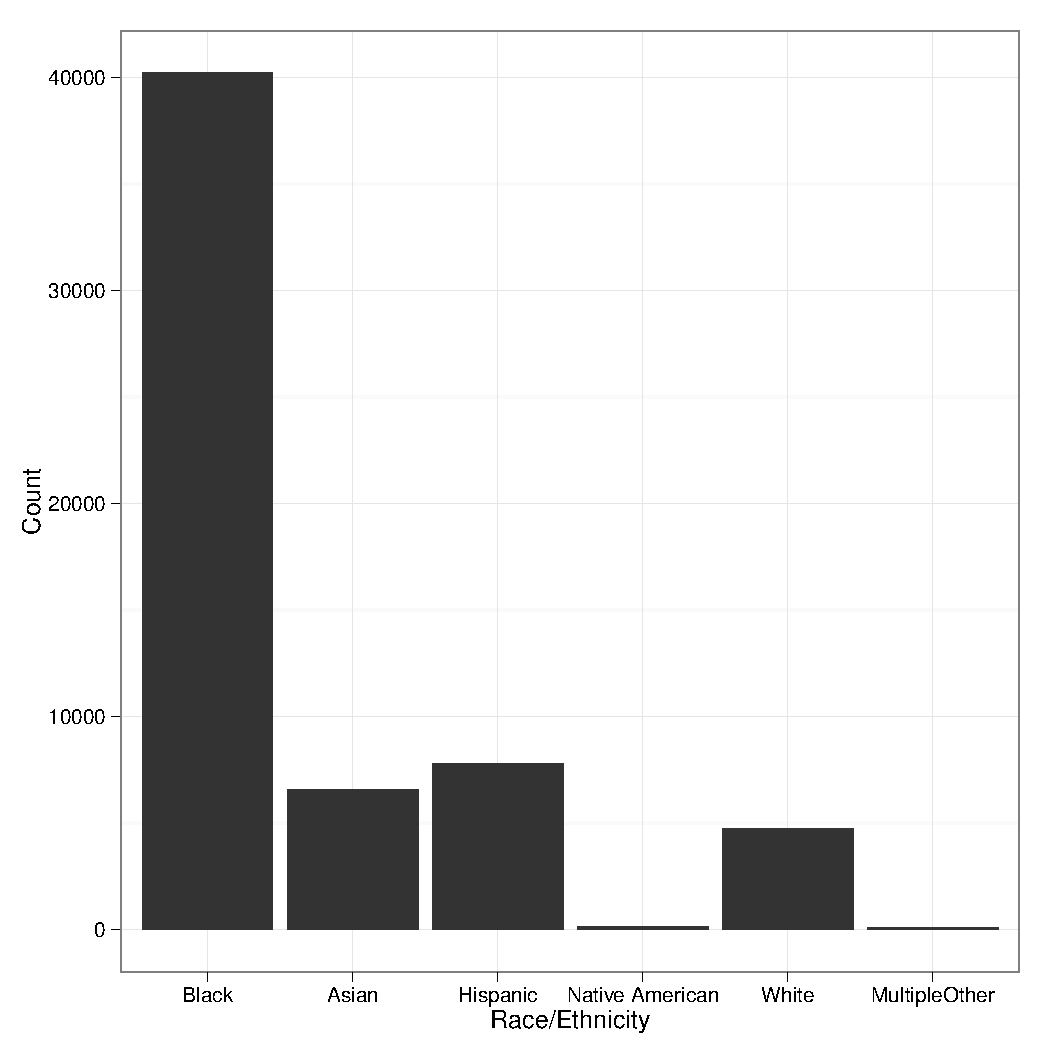
\includegraphics[width=.75\textwidth,height=.35\paperheight]{figure/unnamed-chunk-9} \hfill{}

\caption[Graphic]{Graphic\label{fig:unnamed-chunk-9}}
\end{figure}

\end{knitrout}


\subsection{Consistent Value of race\_ethnicity}

First, create a variable indicating how many unique values race\_ethnicity assumes for each student called nvals\_race.




\begin{knitrout}
\definecolor{shadecolor}{rgb}{0.969, 0.969, 0.969}\color{fgcolor}\begin{kframe}
\begin{flushleft}
\ttfamily\noindent
\hlcomment{\usebox{\hlnormalsizeboxhash}{\ }Get{\ }number{\ }of{\ }unique{\ }values{\ }by{\ }sid}\hspace*{\fill}\\
\hlstd{}\hlsymbol{nvals}{\ }\hlassignement{\usebox{\hlnormalsizeboxlessthan}-}{\ }\hlfunctioncall{tapply}\hlkeyword{(}\hlsymbol{stuatt}\hlkeyword{\usebox{\hlnormalsizeboxdollar}}\hlsymbol{race\usebox{\hlnormalsizeboxunderscore}ethnicity}\hlkeyword{,}{\ }\hlsymbol{stuatt}\hlkeyword{\usebox{\hlnormalsizeboxdollar}}\hlsymbol{sid}\hlkeyword{,}{\ }\hlkeyword{function}\hlkeyword{(}\hlformalargs{x}\hlkeyword{)}{\ }\hlfunctioncall{length}\hlkeyword{(}\hlfunctioncall{unique}\hlkeyword{(}\hlsymbol{x}\hlkeyword{)}\hlkeyword{)}\hlkeyword{)}\hspace*{\fill}\\
\hlstd{}\hlfunctioncall{table}\hlkeyword{(}\hlsymbol{nvals}\hlkeyword{)}\mbox{}
\normalfont
\end{flushleft}
\begin{verbatim}
nvals
    1     2     3 
16237   149     5 
\end{verbatim}
\end{kframe}
\end{knitrout}


\begin{knitrout}
\definecolor{shadecolor}{rgb}{0.969, 0.969, 0.969}\color{fgcolor}\begin{kframe}
\begin{flushleft}
\ttfamily\noindent
\hlfunctioncall{library}\hlkeyword{(}\hlsymbol{ggplot2}\hlkeyword{)}\hspace*{\fill}\\
\hlstd{}\hlfunctioncall{qplot}\hlkeyword{(}\hlfunctioncall{as.factor}\hlkeyword{(}\hlsymbol{nvals}\hlkeyword{)}\hlkeyword{,}{\ }\hlargument{geom}{\ }\hlargument{=}{\ }\hlstring{"{}bar"{}}\hlkeyword{)}{\ }\hlkeyword{+}{\ }\hlfunctioncall{theme\usebox{\hlnormalsizeboxunderscore}bw}\hlkeyword{(}\hlkeyword{)}{\ }\hlkeyword{+}{\ }\hlfunctioncall{xlab}\hlkeyword{(}\hlstring{"{}Unique{\ }Race{\ }Codes"{}}\hlkeyword{)}{\ }\hlkeyword{+}\hspace*{\fill}\\
\hlstd{}{\ }{\ }{\ }{\ }\hlfunctioncall{ylab}\hlkeyword{(}\hlstring{"{}Count"{}}\hlkeyword{)}\mbox{}
\normalfont
\end{flushleft}
\end{kframe}\begin{figure}[]


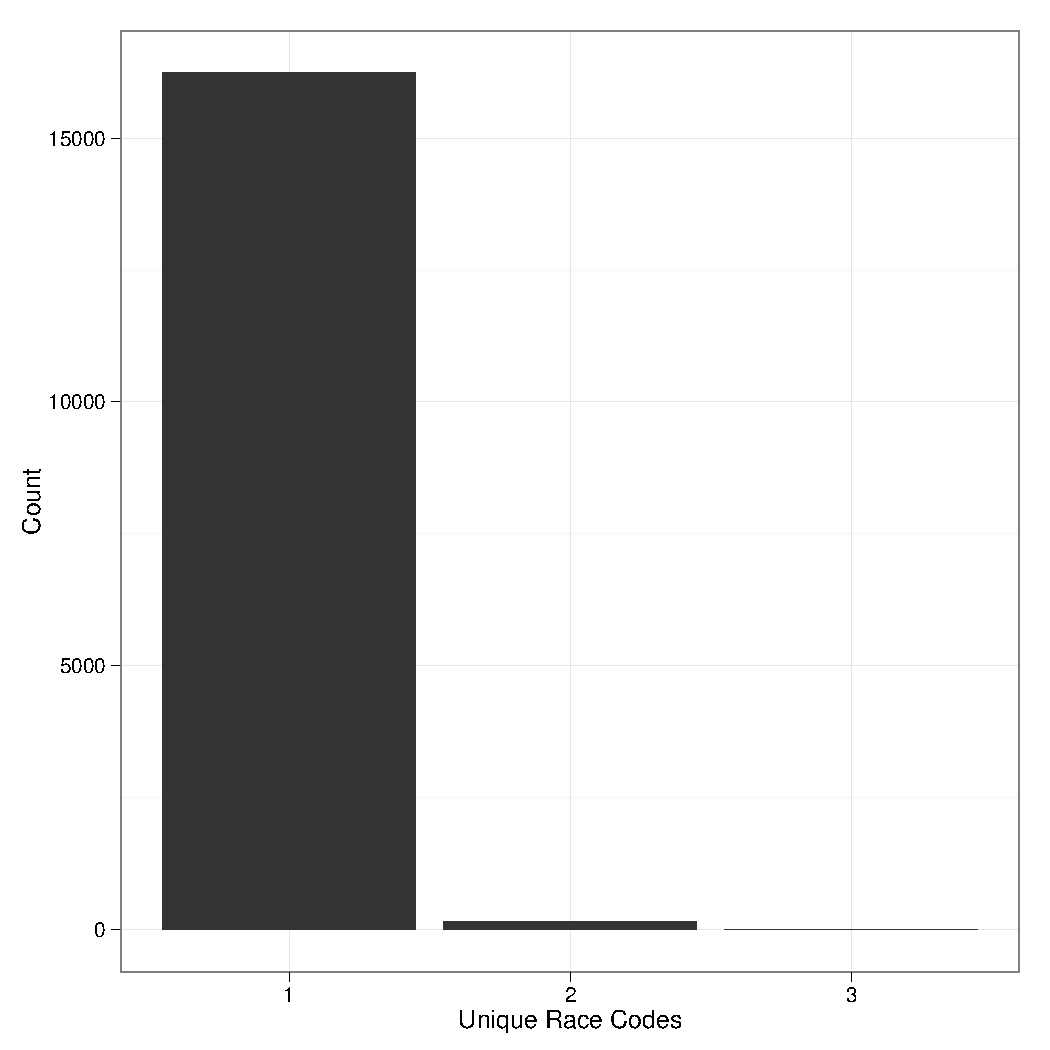
\includegraphics[width=.75\textwidth,height=.35\paperheight]{figure/unnamed-chunk-11} \hfill{}

\caption[Graphic 2]{Graphic 2\label{fig:unnamed-chunk-11}}
\end{figure}

\end{knitrout}


Next, for students with more than one value for race\_ethnicity, assign the modal value as the student's race.

\begin{knitrout}
\definecolor{shadecolor}{rgb}{0.969, 0.969, 0.969}\color{fgcolor}\begin{kframe}
\begin{flushleft}
\ttfamily\noindent
\hlcomment{\usebox{\hlnormalsizeboxhash}{\ }First{\ }we{\ }need{\ }to{\ }create{\ }a{\ }\usebox{\hlnormalsizeboxsinglequote}mode\usebox{\hlnormalsizeboxsinglequote}{\ }function{\ }in{\ }R{\ }that{\ }mimics{\ }Stata{\ }statamode}\hspace*{\fill}\\
\hlstd{}\hlcomment{\usebox{\hlnormalsizeboxhash}{\ }creates{\ }a{\ }list{\ }of{\ }the{\ }modal{\ }values{\ }and{\ }assigns{\ }\usebox{\hlnormalsizeboxsinglequote}.\usebox{\hlnormalsizeboxsinglequote}{\ }{\ }If{\ }more{\ }than{\ }one{\ }mode}\hspace*{\fill}\\
\hlstd{}\hlcomment{\usebox{\hlnormalsizeboxhash}{\ }exists}\hspace*{\fill}\\
\hlstd{}\hlsymbol{statamode}{\ }\hlassignement{\usebox{\hlnormalsizeboxlessthan}-}{\ }\hlkeyword{function}\hlkeyword{(}\hlformalargs{x}\hlkeyword{)}{\ }\hlkeyword{\usebox{\hlnormalsizeboxopenbrace}}\hspace*{\fill}\\
\hlstd{}{\ }{\ }{\ }{\ }\hlsymbol{z}{\ }\hlassignement{\usebox{\hlnormalsizeboxlessthan}-}{\ }\hlfunctioncall{table}\hlkeyword{(}\hlfunctioncall{as.vector}\hlkeyword{(}\hlsymbol{x}\hlkeyword{)}\hlkeyword{)}\hspace*{\fill}\\
\hlstd{}{\ }{\ }{\ }{\ }\hlsymbol{m}{\ }\hlassignement{\usebox{\hlnormalsizeboxlessthan}-}{\ }\hlfunctioncall{names}\hlkeyword{(}\hlsymbol{z}\hlkeyword{)}\hlkeyword{[}\hlsymbol{z}{\ }=={\ }\hlfunctioncall{max}\hlkeyword{(}\hlsymbol{z}\hlkeyword{)}\hlkeyword{]}\hspace*{\fill}\\
\hlstd{}{\ }{\ }{\ }{\ }\hlkeyword{if}{\ }\hlkeyword{(}\hlfunctioncall{length}\hlkeyword{(}\hlsymbol{m}\hlkeyword{)}{\ }=={\ }\hlnumber{1}\hlkeyword{)}{\ }\hlkeyword{\usebox{\hlnormalsizeboxopenbrace}}\hspace*{\fill}\\
\hlstd{}{\ }{\ }{\ }{\ }{\ }{\ }{\ }{\ }\hlfunctioncall{return}\hlkeyword{(}\hlsymbol{m}\hlkeyword{)}\hspace*{\fill}\\
\hlstd{}{\ }{\ }{\ }{\ }\hlkeyword{\usebox{\hlnormalsizeboxclosebrace}}\hspace*{\fill}\\
\hlstd{}{\ }{\ }{\ }{\ }\hlsymbol{return}\hlfunctioncall{}\hlkeyword{(}\hlstring{"{}."{}}\hlkeyword{)}\hspace*{\fill}\\
\hlstd{}\hlkeyword{\usebox{\hlnormalsizeboxclosebrace}}\hspace*{\fill}\\
\hlstd{}\hspace*{\fill}\\
\hlstd{}\hlcomment{\usebox{\hlnormalsizeboxhash}{\ }Create{\ }new{\ }data{\ }frame{\ }for{\ }individual{\ }student{\ }Create{\ }nvals{\ }while{\ }we{\ }are{\ }at{\ }it}\hspace*{\fill}\\
\hlstd{}\hlfunctioncall{library}\hlkeyword{(}\hlsymbol{plyr}\hlkeyword{)}{\ }{\ }\hlcomment{\usebox{\hlnormalsizeboxhash}{\ }convenience{\ }functions{\ }for{\ }summarizing{\ }data{\ }in{\ }R}\hspace*{\fill}\\
\hlstd{}\hlsymbol{modes}{\ }\hlassignement{\usebox{\hlnormalsizeboxlessthan}-}{\ }\hlfunctioncall{ddply}\hlkeyword{(}\hlsymbol{stuatt}\hlkeyword{,}{\ }\hlfunctioncall{.}\hlkeyword{(}\hlsymbol{sid}\hlkeyword{)}\hlkeyword{,}{\ }\hlsymbol{summarize}\hlkeyword{,}{\ }\hlargument{race\usebox{\hlnormalsizeboxunderscore}temp}{\ }\hlargument{=}{\ }\hlfunctioncall{statamode}\hlkeyword{(}\hlsymbol{race\usebox{\hlnormalsizeboxunderscore}ethnicity}\hlkeyword{)}\hlkeyword{,}\hspace*{\fill}\\
\hlstd{}{\ }{\ }{\ }{\ }\hlargument{nvals}{\ }\hlargument{=}{\ }\hlfunctioncall{length}\hlkeyword{(}\hlfunctioncall{unique}\hlkeyword{(}\hlsymbol{race\usebox{\hlnormalsizeboxunderscore}ethnicity}\hlkeyword{)}\hlkeyword{)}\hlkeyword{)}\hspace*{\fill}\\
\hlstd{}\hlsymbol{tab1}{\ }\hlassignement{\usebox{\hlnormalsizeboxlessthan}-}{\ }\hlfunctioncall{table}\hlkeyword{(}\hlsymbol{modes}\hlkeyword{\usebox{\hlnormalsizeboxdollar}}\hlsymbol{race\usebox{\hlnormalsizeboxunderscore}temp}\hlkeyword{,}{\ }\hlsymbol{modes}\hlkeyword{\usebox{\hlnormalsizeboxdollar}}\hlsymbol{nvals}\hlkeyword{)}\hspace*{\fill}\\
\hlstd{}\hlfunctioncall{addmargins}\hlkeyword{(}\hlsymbol{tab1}\hlkeyword{,}{\ }\hlargument{FUN}{\ }\hlargument{=}{\ }\hlfunctioncall{list}\hlkeyword{(}\hlargument{Total}{\ }\hlargument{=}{\ }\hlsymbol{sum}\hlkeyword{)}\hlkeyword{,}{\ }\hlargument{quiet}{\ }\hlargument{=}{\ }\hlnumber{TRUE}\hlkeyword{)}\mbox{}
\normalfont
\end{flushleft}
\begin{verbatim}
                 
                      1     2     3 Total
  .                   0    28     1    29
  Asian            1924    21     0  1945
  Black           10576    35     2 10613
  Hispanic         2396    14     0  2410
  MultipleOther      20     6     0    26
  Native American     7    29     2    38
  White            1314    16     0  1330
  Total           16237   149     5 16391
\end{verbatim}
\end{kframe}
\end{knitrout}


Check:  What does the distribution of the temporary race variable look like for students with only one unique race value and for 
students with more than one race value?

\begin{knitrout}
\definecolor{shadecolor}{rgb}{0.969, 0.969, 0.969}\color{fgcolor}\begin{kframe}
\begin{flushleft}
\ttfamily\noindent
\hlsymbol{df}{\ }\hlassignement{\usebox{\hlnormalsizeboxlessthan}-}{\ }\hlfunctioncall{as.data.frame}\hlkeyword{(}\hlsymbol{tab1}\hlkeyword{)}\hspace*{\fill}\\
\hlstd{}\hlfunctioncall{qplot}\hlkeyword{(}\hlsymbol{Var1}\hlkeyword{,}{\ }\hlsymbol{Var2}\hlkeyword{,}{\ }\hlargument{geom}{\ }\hlargument{=}{\ }\hlstring{"{}point"{}}\hlkeyword{,}{\ }\hlargument{size}{\ }\hlargument{=}{\ }\hlsymbol{Freq}\hlkeyword{,}{\ }\hlargument{data}{\ }\hlargument{=}{\ }\hlsymbol{df}\hlkeyword{)}{\ }\hlkeyword{+}{\ }\hlfunctioncall{theme\usebox{\hlnormalsizeboxunderscore}bw}\hlkeyword{(}\hlkeyword{)}{\ }\hlkeyword{+}\hspace*{\fill}\\
\hlstd{}{\ }{\ }{\ }{\ }\hlfunctioncall{xlab}\hlkeyword{(}\hlstring{"{}Nvals"{}}\hlkeyword{)}{\ }\hlkeyword{+}{\ }\hlfunctioncall{ylab}\hlkeyword{(}\hlstring{"{}Modal{\ }Race"{}}\hlkeyword{)}\mbox{}
\normalfont
\end{flushleft}
\end{kframe}\begin{figure}[]


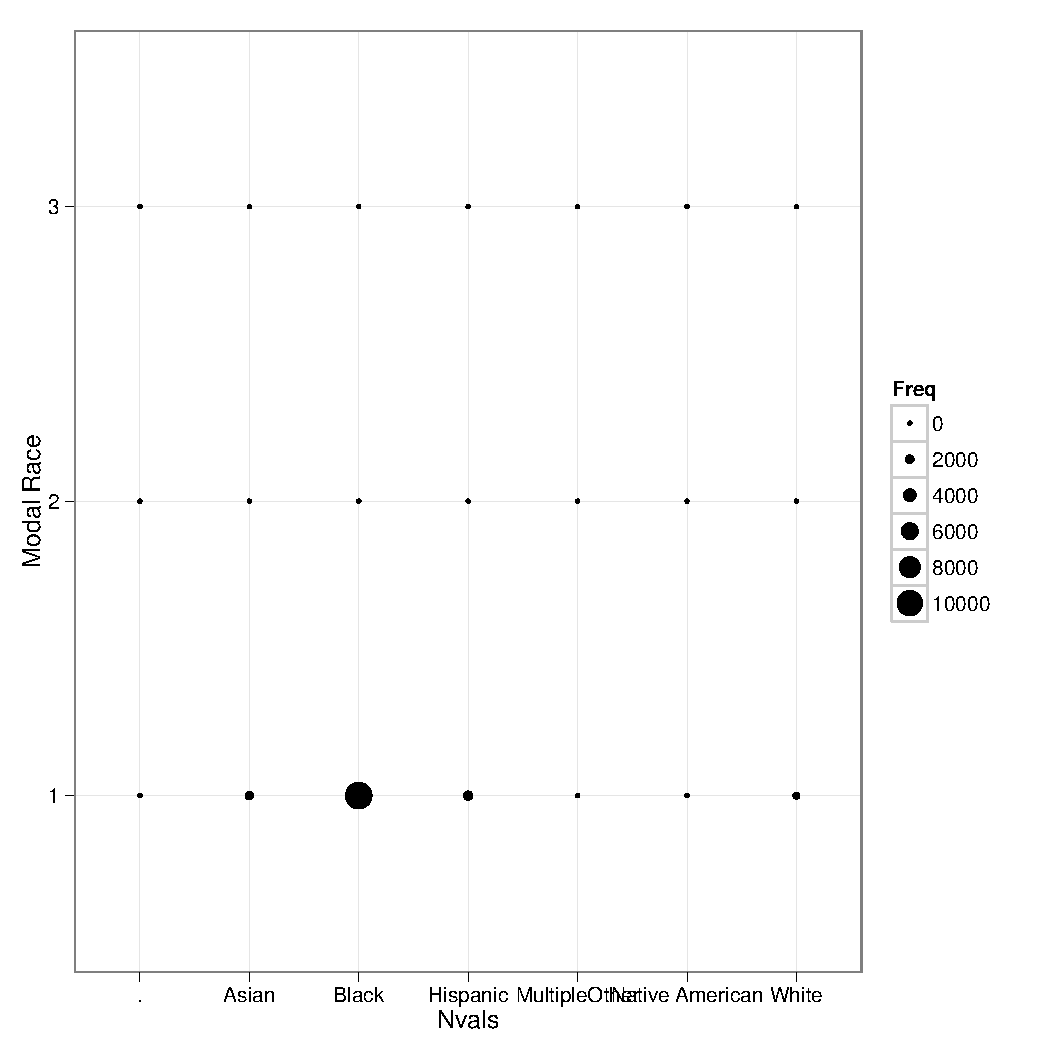
\includegraphics[width=.95\textwidth,height=.2\paperheight]{figure/dotplot} \hfill{}

\caption[Graphic 2]{Graphic 2\label{fig:dotplot}}
\end{figure}

\end{knitrout}



C. It appears that we now have 29 students with appended values for the race\_temp variable. This occurs because these students'
race\_ethnicity has two or more modes, so none of the modes is selected as the variable mode in part B of this step.  For these 
students, assign their most recently observed race value as their race\_ethnicity.

\begin{knitrout}
\definecolor{shadecolor}{rgb}{0.969, 0.969, 0.969}\color{fgcolor}\begin{kframe}
\begin{flushleft}
\ttfamily\noindent
\hlcomment{\usebox{\hlnormalsizeboxhash}{\ }Create{\ }a{\ }variable{\ }indicating{\ }the{\ }latest{\ }school{\ }year}\hspace*{\fill}\\
\hlstd{}\hlsymbol{modes}{\ }\hlassignement{\usebox{\hlnormalsizeboxlessthan}-}{\ }\hlsymbol{modes}{\ }\hlassignement{\usebox{\hlnormalsizeboxlessthan}-}{\ }\hlfunctioncall{ddply}\hlkeyword{(}\hlsymbol{stuatt}\hlkeyword{,}{\ }\hlfunctioncall{.}\hlkeyword{(}\hlsymbol{sid}\hlkeyword{)}\hlkeyword{,}{\ }\hlsymbol{summarize}\hlkeyword{,}{\ }\hlargument{race\usebox{\hlnormalsizeboxunderscore}temp}{\ }\hlargument{=}{\ }\hlfunctioncall{statamode}\hlkeyword{(}\hlsymbol{race\usebox{\hlnormalsizeboxunderscore}ethnicity}\hlkeyword{)}\hlkeyword{,}\hspace*{\fill}\\
\hlstd{}{\ }{\ }{\ }{\ }\hlargument{nvals}{\ }\hlargument{=}{\ }\hlfunctioncall{length}\hlkeyword{(}\hlfunctioncall{unique}\hlkeyword{(}\hlsymbol{race\usebox{\hlnormalsizeboxunderscore}ethnicity}\hlkeyword{)}\hlkeyword{)}\hlkeyword{,}{\ }\hlargument{most\usebox{\hlnormalsizeboxunderscore}recent\usebox{\hlnormalsizeboxunderscore}year}{\ }\hlargument{=}{\ }\hlfunctioncall{max}\hlkeyword{(}\hlsymbol{school\usebox{\hlnormalsizeboxunderscore}year}\hlkeyword{)}\hlkeyword{,}\hspace*{\fill}\\
\hlstd{}{\ }{\ }{\ }{\ }\hlargument{most\usebox{\hlnormalsizeboxunderscore}recent\usebox{\hlnormalsizeboxunderscore}race}{\ }\hlargument{=}{\ }\hlfunctioncall{tail}\hlkeyword{(}\hlsymbol{race\usebox{\hlnormalsizeboxunderscore}ethnicity}\hlkeyword{,}{\ }\hlnumber{1}\hlkeyword{)}\hlkeyword{)}\hspace*{\fill}\\
\hlstd{}\hlsymbol{modes}\hlkeyword{\usebox{\hlnormalsizeboxdollar}}\hlsymbol{race2}\hlkeyword{[}\hlsymbol{modes}\hlkeyword{\usebox{\hlnormalsizeboxdollar}}\hlsymbol{race\usebox{\hlnormalsizeboxunderscore}temp}{\ }\hlkeyword{!=}{\ }\hlstring{"{}."{}}\hlkeyword{]}{\ }\hlassignement{\usebox{\hlnormalsizeboxlessthan}-}{\ }\hlsymbol{modes}\hlkeyword{\usebox{\hlnormalsizeboxdollar}}\hlsymbol{race\usebox{\hlnormalsizeboxunderscore}temp}\hlkeyword{[}\hlsymbol{modes}\hlkeyword{\usebox{\hlnormalsizeboxdollar}}\hlsymbol{race\usebox{\hlnormalsizeboxunderscore}temp}{\ }\hlkeyword{!=}\hspace*{\fill}\\
\hlstd{}{\ }{\ }{\ }{\ }\hlstring{"{}."{}}\hlkeyword{]}\hspace*{\fill}\\
\hlstd{}\hlsymbol{modes}\hlkeyword{\usebox{\hlnormalsizeboxdollar}}\hlsymbol{race2}\hlkeyword{[}\hlsymbol{modes}\hlkeyword{\usebox{\hlnormalsizeboxdollar}}\hlsymbol{race\usebox{\hlnormalsizeboxunderscore}temp}{\ }=={\ }\hlstring{"{}."{}}\hlkeyword{]}{\ }\hlassignement{\usebox{\hlnormalsizeboxlessthan}-}{\ }\hlfunctioncall{as.character}\hlkeyword{(}\hlsymbol{modes}\hlkeyword{\usebox{\hlnormalsizeboxdollar}}\hlsymbol{most\usebox{\hlnormalsizeboxunderscore}recent\usebox{\hlnormalsizeboxunderscore}race}\hlkeyword{[}\hlsymbol{modes}\hlkeyword{\usebox{\hlnormalsizeboxdollar}}\hlsymbol{race\usebox{\hlnormalsizeboxunderscore}temp}{\ }==\hspace*{\fill}\\
\hlstd{}{\ }{\ }{\ }{\ }\hlstring{"{}."{}}\hlkeyword{]}\hlkeyword{)}\hspace*{\fill}\\
\hlstd{}\hlfunctioncall{head}\hlkeyword{(}\hlsymbol{modes}\hlkeyword{)}\mbox{}
\normalfont
\end{flushleft}
\begin{verbatim}
  sid race_temp nvals most_recent_year most_recent_race    race2
1   1  Hispanic     2             2007         Hispanic Hispanic
2   2         .     2             2007            Black    Black
3   3     Black     2             2007            Black    Black
4   4     Black     1             2007            Black    Black
5   5     Black     1             2007            Black    Black
6   7     Black     1             2001            Black    Black
\end{verbatim}
\begin{flushleft}
\ttfamily\noindent
\hlcomment{\usebox{\hlnormalsizeboxhash}{\ }Delete{\ }old{\ }vars{\ }on{\ }stuatt}\hspace*{\fill}\\
\hlstd{}\hlsymbol{stuatt}{\ }\hlassignement{\usebox{\hlnormalsizeboxlessthan}-}{\ }\hlfunctioncall{subset}\hlkeyword{(}\hlsymbol{stuatt}\hlkeyword{,}{\ }\hlargument{select}{\ }\hlargument{=}{\ }\hlfunctioncall{c}\hlkeyword{(}\hlstring{"{}sid"{}}\hlkeyword{,}{\ }\hlstring{"{}school\usebox{\hlnormalsizeboxunderscore}year"{}}\hlkeyword{,}{\ }\hlstring{"{}race\usebox{\hlnormalsizeboxunderscore}ethnicity"{}}\hlkeyword{)}\hlkeyword{)}\hspace*{\fill}\\
\hlstd{}\hlcomment{\usebox{\hlnormalsizeboxhash}{\ }Assign{\ }the{\ }value{\ }associated{\ }with{\ }the{\ }most{\ }recent{\ }year{\ }as{\ }the{\ }permanent}\hspace*{\fill}\\
\hlstd{}\hlcomment{\usebox{\hlnormalsizeboxhash}{\ }race\usebox{\hlnormalsizeboxunderscore}ethnicity{\ }for{\ }the{\ }students{\ }with{\ }missing{\ }race}\hspace*{\fill}\\
\hlstd{}\hlsymbol{stuatt}{\ }\hlassignement{\usebox{\hlnormalsizeboxlessthan}-}{\ }\hlfunctioncall{merge}\hlkeyword{(}\hlsymbol{stuatt}\hlkeyword{,}{\ }\hlsymbol{modes}\hlkeyword{)}\hspace*{\fill}\\
\hlstd{}\hlfunctioncall{rm}\hlkeyword{(}\hlsymbol{modes}\hlkeyword{)}\hspace*{\fill}\\
\hlstd{}\hlsymbol{stuatt}\hlkeyword{\usebox{\hlnormalsizeboxdollar}}\hlsymbol{race\usebox{\hlnormalsizeboxunderscore}ethnicity}{\ }\hlassignement{\usebox{\hlnormalsizeboxlessthan}-}{\ }\hlsymbol{stuatt}\hlkeyword{\usebox{\hlnormalsizeboxdollar}}\hlsymbol{race2}\hspace*{\fill}\\
\hlstd{}\hlsymbol{stuatt}{\ }\hlassignement{\usebox{\hlnormalsizeboxlessthan}-}{\ }\hlfunctioncall{subset}\hlkeyword{(}\hlsymbol{stuatt}\hlkeyword{,}{\ }\hlargument{select}{\ }\hlargument{=}{\ }\hlfunctioncall{c}\hlkeyword{(}\hlstring{"{}sid"{}}\hlkeyword{,}{\ }\hlstring{"{}school\usebox{\hlnormalsizeboxunderscore}year"{}}\hlkeyword{,}{\ }\hlstring{"{}race\usebox{\hlnormalsizeboxunderscore}ethnicity"{}}\hlkeyword{)}\hlkeyword{)}\hspace*{\fill}\\
\hlstd{}\hlfunctioncall{head}\hlkeyword{(}\hlsymbol{stuatt}\hlkeyword{,}{\ }\hlargument{n}{\ }\hlargument{=}{\ }\hlnumber{20}\hlkeyword{)}\mbox{}
\normalfont
\end{flushleft}
\begin{verbatim}
   sid school_year race_ethnicity
1    1        2004       Hispanic
2    1        2005       Hispanic
3    1        2006       Hispanic
4    1        2007       Hispanic
5    2        2006          Black
6    2        2007          Black
7    3        2005          Black
8    3        2006          Black
9    3        2007          Black
10   4        2005          Black
11   4        2006          Black
12   4        2007          Black
13   5        2007          Black
14   7        2001          Black
15   8        2001          Black
16   9        2001          Black
17   9        2002          Black
18  11        2001          Black
19  11        2002          Black
20  11        2003          Black
\end{verbatim}
\end{kframe}
\end{knitrout}


Check: What is the distribution of the race\_ethnicity in the final file? If all steps were completed correctly, the distributions 
should look exactly the same as in the Check steps for the final  race\_ethnicity variable in 3C.

\begin{knitrout}
\definecolor{shadecolor}{rgb}{0.969, 0.969, 0.969}\color{fgcolor}\begin{kframe}
\begin{flushleft}
\ttfamily\noindent
\hlfunctioncall{qplot}\hlkeyword{(}\hlsymbol{race\usebox{\hlnormalsizeboxunderscore}ethnicity}\hlkeyword{,}{\ }\hlargument{data}{\ }\hlargument{=}{\ }\hlsymbol{stuatt}\hlkeyword{,}{\ }\hlargument{geom}{\ }\hlargument{=}{\ }\hlstring{"{}histogram"{}}\hlkeyword{)}{\ }\hlkeyword{+}{\ }\hlfunctioncall{theme\usebox{\hlnormalsizeboxunderscore}bw}\hlkeyword{(}\hlkeyword{)}{\ }\hlkeyword{+}\hspace*{\fill}\\
\hlstd{}{\ }{\ }{\ }{\ }\hlfunctioncall{stat\usebox{\hlnormalsizeboxunderscore}bin}\hlkeyword{(}\hlargument{geom}{\ }\hlargument{=}{\ }\hlstring{"{}text"{}}\hlkeyword{,}{\ }\hlfunctioncall{aes}\hlkeyword{(}\hlargument{label}{\ }\hlargument{=}{\ }\hlsymbol{..count..}\hlkeyword{,}{\ }\hlargument{vjust}{\ }\hlargument{=}{\ }\hlkeyword{-}\hlnumber{0.5}\hlkeyword{)}\hlkeyword{)}\mbox{}
\normalfont
\end{flushleft}
\begin{verbatim}
## ymax not defined: adjusting position using y instead
\end{verbatim}
\end{kframe}\begin{figure}[]


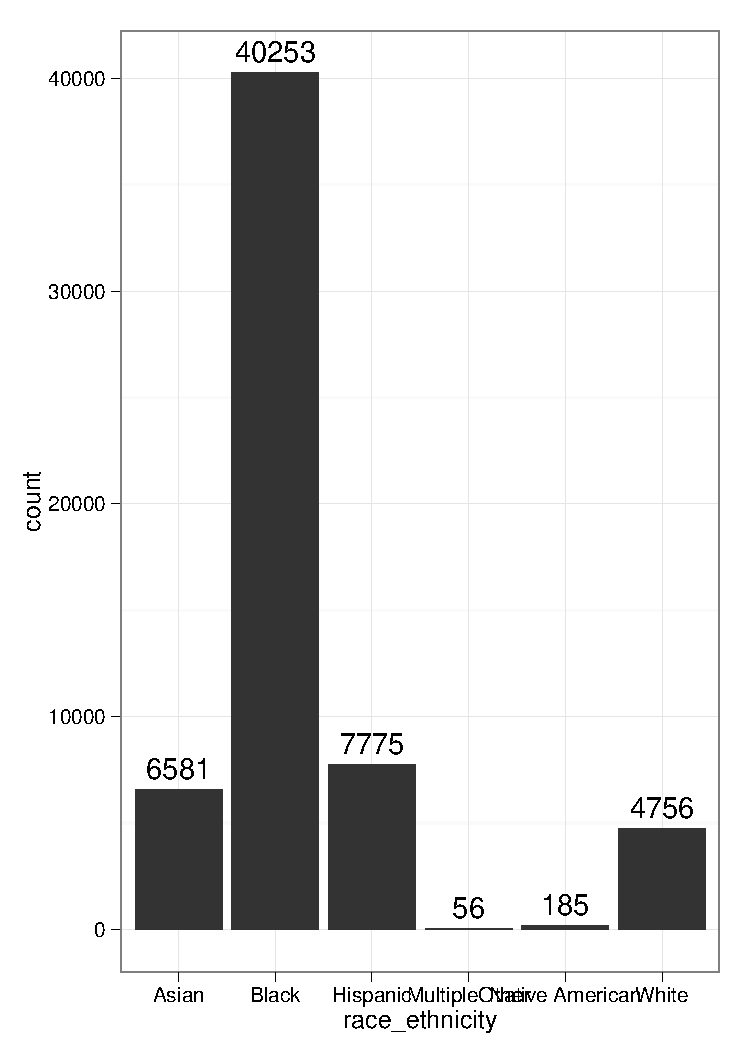
\includegraphics[width=.7\textwidth,height=.4\paperheight]{figure/histogramfinal} \hfill{}

\caption[Graphic 3]{Graphic 3\label{fig:histogramfinal}}
\end{figure}

\end{knitrout}


\end{document}


